\chapter{Background and Theoretical Foundations}

\section{Introduction}

This chapter provides an overview of the concepts needed to develop and analyze \ac{RAG} pipelines used in this thesis. It does NOT address how to train or tune the parameterization of a language model. Rather, it focuses on the aspects most directly related to the inference time of an \ac{RAG} system.

It begins with a description of \acp{LLM}. This explains the Transformer architecture in practical terms. Additionally, although training, fine tuning, prompt engineering, and training from scratch are addressed in the chapter as paradigms for developing \acp{LLM}, they are described such that can be distinguished from the retrieval level and system level methods which are being developed in this project. Next, \acp{RAG} are more thoroughly described, the process flow of \ac{RAG}, retrieval approaches and other sophisticated retrieval techniques examined in the project source code. Lastly, the chapter provides an overview of \ac{HPC} hardware configurations and discuss the common metrics applied to measure performance, retrieval accuracy, and quality of output.

\section{Large Language Models (LLMs)}

\subsection{Overview}

\acp{LLM} are deep learning-based language models which enable processing and generating natural language. Generally these models are trained on massive datasets of text data and statistically learn relationships in natural language, including word, phrase, concept, and context relationships. Due to the nature of their training, \acp{LLM} can be utilized for various applications, including question-answering (QA), document summarization, text generation, and extracting information from documents without explicit task-oriented programming.

While the effectiveness of using \acp{LLM} for real-world applications is directly influenced by the model itself; however, there are numerous factors that influence the effectiveness of the model within a larger system architecture. When utilizing \acp{LLM}, each time an inference operation is requested, the user provides an input query or prompt. After receiving the input prompt, the model processes the prompt layer-by-layer (many times) through a series of transformer layers and generates output tokens one at a time. While not all operations require significant computational resources, operations involving longer prompts or multiple simultaneous requests may consume considerable resources. Consequently, there are several system level considerations that can have a substantial impact on the performance experienced by users of \ac{LLM}-based systems. These include batching input requests together, caching intermediate results, selecting appropriate hardware and designing the retrieval mechanism.

This research focuses on utilizing an \ac{LLM} as part of a \ac{RAG} system. Therefore, while the primary experimental focus will not involve improving the weights within the \acp{LLM}; rather, it involves examining how different approaches to retrieving additional contextual information and overall system configurations effect both the quality and efficiency of the final generated answer.

\subsection{Transformer Architecture}

\begin{figure}[t]
    \centering
    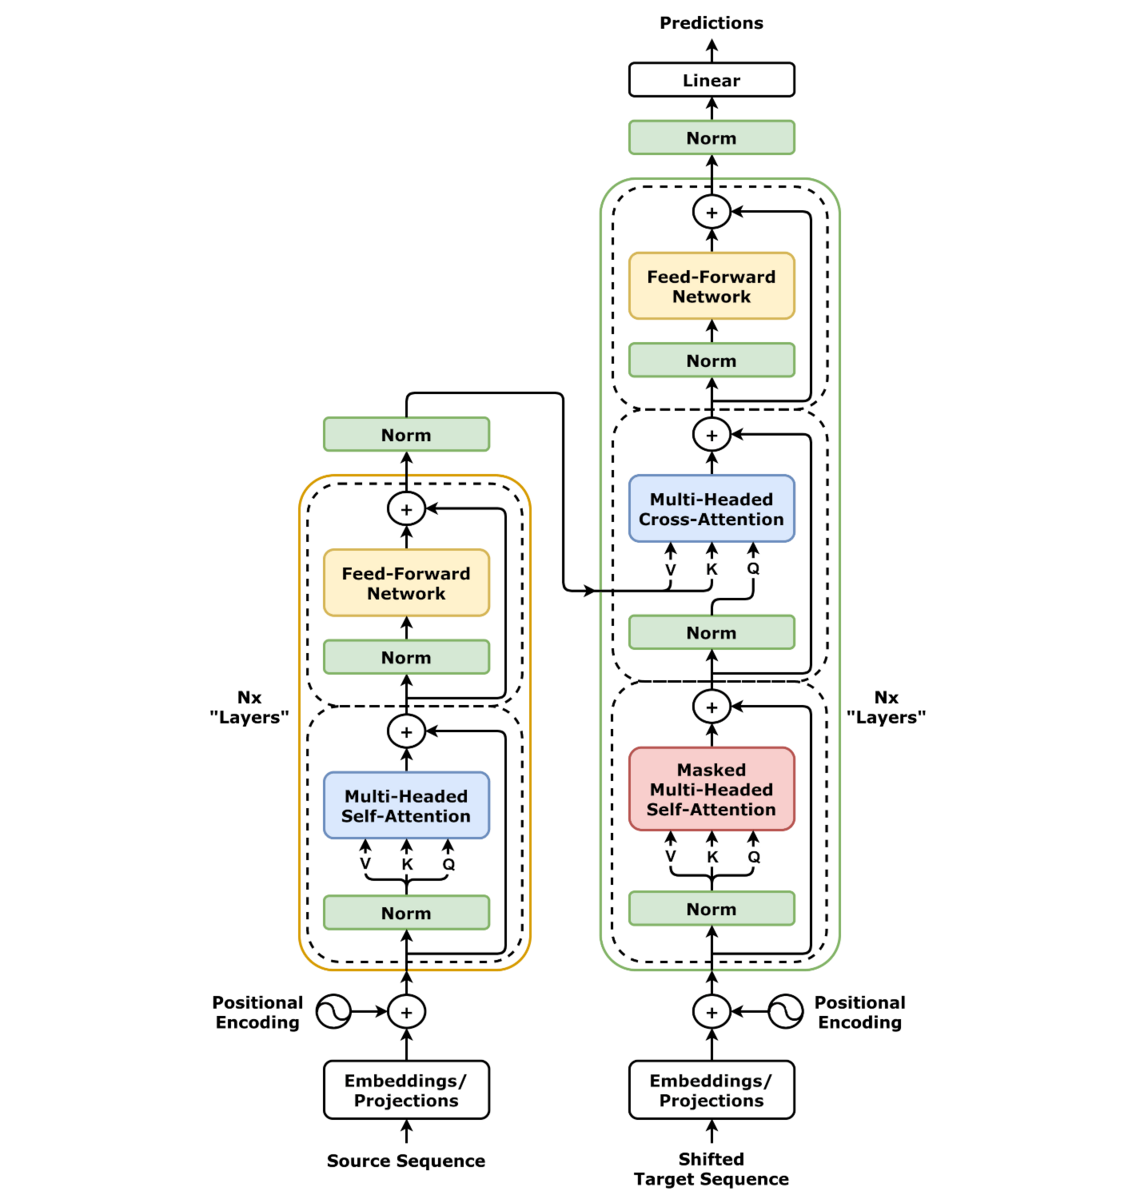
\includegraphics[width=\textwidth]{images/Transformer,_full_architecture.png}
    \caption[Transformer encoder--decoder architecture]{Transformer encoder--decoder architecture. The diagram shows the main building blocks used to transform input tokens into contextual representations and generated output tokens.}
    \label{fig:transformer-architecture}
\end{figure}

Modern \acp{LLM} are build upon the Transformer architecture introduced by Vaswani \emph{et al.} \cite{vaswani2017attention}. The transformer architecture may be viewed as a sequential processing model, where a sequence of tokens is read into the model, and the representation of each token is iteratively updated based on the representations of the surrounding tokens. This is significantly different from earlier recurrent models that were primarily sequential in their operation, and therefore lacked much inherent or explicit parallelism.   

The most important idea in the Transformer is \emph{self-attention}. In simple terms, self-attention is the mechanism that helps the model decide which words in the input are important for understanding each other. For example, in the sentence ``the server restarted because it ran out of memory'', the word ``it'' should be linked more strongly to ``server'' than to unrelated words. Self-attention allows the model to make these links automatically. Each token is compared with the other tokens in the sequence, and the model gives higher weight to tokens that provide useful context.

More technically, the model creates three learned representations for each token: a query ($Q$), a key ($K$), and a value ($V$). The query represents what a token is looking for, the key represents what each token offers, and the value contains the information that will be passed forward if that token is considered relevant. The attention score is calculated as:
\begin{equation}
    \mathrm{Attention}(Q, K, V) = \mathrm{softmax}\left( \frac{QK^{\top}}{\sqrt{d_k}} \right) V,
\end{equation}
where $d_k$ is the dimensionality of the key vectors. The softmax operation converts similarity scores into weights, and these weights determine how much information from each token is included in the updated representation.

The Transformer extends self-attention through \emph{multi-head attention}. Instead of applying attention only once, the model uses several attention heads in parallel. One head may focus on grammatical structure, another may focus on entity relationships, and another may focus on long-distance dependencies. The outputs of the heads are then combined. This gives the model a richer representation of the input than a single attention calculation would provide.

\begin{figure}[H]
    \centering
    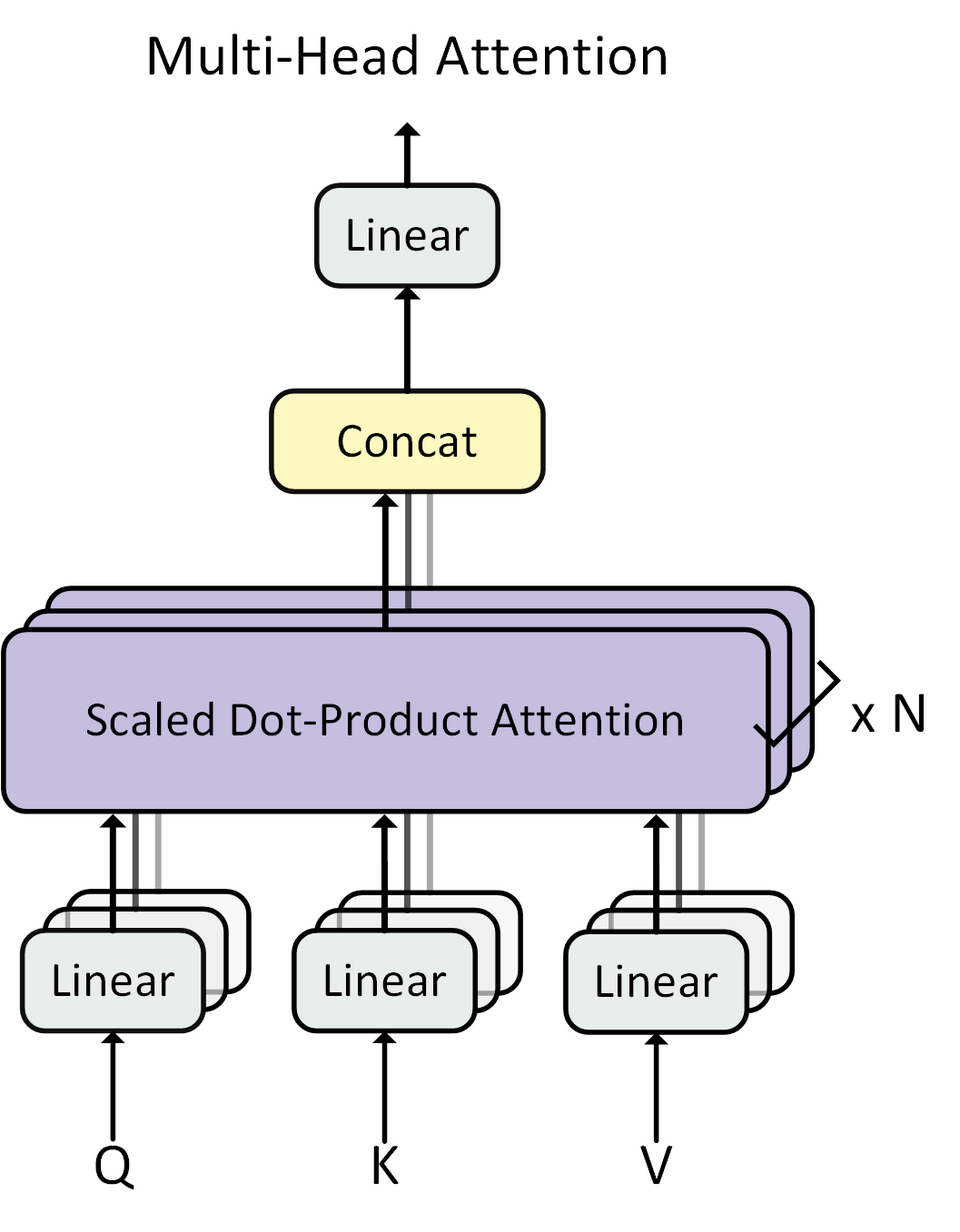
\includegraphics[width=0.75\linewidth]{images/Multi-head_attention.png}
    \caption{Multi-head attention mechanism, illustrating the linear projections of queries, keys, and values, followed by parallel attention heads and concatenation. Adapted from Alammar~\cite{alammar2018transformer}.}
    \label{fig:multihead-attention}
\end{figure}

The most important aspect of how the Transformer affects the way it behaves during inference, is through its influence on generation. Typically, when using a model for generating something (such as an answer), the generation process is done in a sequential manner. That means the model will produce one item at a time. Therefore, long prompts, large amounts of data that have been retrieved, and/or multiple questions asked could potentially slow down the overall generation process. So, the \ac{RAG} evaluation should consider both if the generated answer was accurate as well as the time taken to generate the answer, the time taken to retrieve the relevant information used by the model to generate the answer, and the total amount of time from start to finish (end-to-end).

\subsection{Development Paradigms and Their Effect on LLM Performance}
\label{subsec:llm_paradigms}

There are several ways to create applications based upon \acp{LLM}. Each application development method has the potential to significantly impact how the model acts and performs within the system. For this research, these methods were discussed in the background section to clearly define what this research was going to investigate. The experiments did not include optimizing models in terms of model size; fine tuning, quantizing, or pruning any models trained prior to running the experiments. The focus of the experiment is on how to best use retrieval strategies and optimize systems in general.

\begin{table}[H]
\caption{LLM development paradigms and their relevance to this thesis.}
\label{tab:llm-development-paradigms}
\centering
\small
\begin{tabularx}{\textwidth}{>{\raggedright\arraybackslash}p{0.22\textwidth}>{\raggedright\arraybackslash}X>{\raggedright\arraybackslash}p{0.25\textwidth}}
\toprule
\textbf{Paradigm} & \textbf{How it affects LLM performance} & \textbf{Role in this thesis} \\
\midrule
Prompt engineering & Changes the instructions and context given to a fixed model. It can improve answer style and task following, but it does not update the model's knowledge. & Background only; prompts are kept controlled across pipeline comparisons. \\
\ac{RAG} & Adds external retrieved context to the prompt. It can improve factual grounding and domain specificity without changing model weights. & Main focus; several retrieval variants are implemented and compared. \\
Fine-tuning & Updates some or all model parameters using task-specific data. It can improve task performance but requires additional training resources and model management. & Out of experimental scope; discussed only to distinguish it from \ac{RAG}. \\
Training from scratch & Learns all model parameters from large datasets. It provides maximum control but requires very large compute, data, and engineering resources. & Out of scope; included only as background. \\
\bottomrule
\end{tabularx}
\end{table}

This distinction is important because retrieval-level techniques improve the information supplied to the model, while model-level techniques modify the model itself. The project contract requires understanding the difference between prompting, \ac{RAG}, fine-tuning, and training from scratch, but the implementation work focuses on deployable \ac{RAG} pipelines and their performance in local and \ac{HPC} environments.


\section{Retrieval-Augmented Generation (RAG)}

\subsection{Concept and Motivation}

\ac{RAG} uses a combination of a language model and an external retriever. In this approach instead of only getting the answer from the language models own parameterized knowledge base it first identifies appropriate passage(s) from a document collection, which are used as additional input to provide contextual support to the language model. Using the \ac{RAG} method has been shown to improve factual grounding and decrease the number of unsupported answers produced by the model especially when the query is specific to a particular domain or type of data that may be less frequently represented within the models' parameterized knowledge base \cite{lewis2020rag}.

In terms of using \ac{RAG} as part of this thesis the reason was largely practical. It's generally easier to update a document collection vs fine tuning/retraining a model. Therefore, a \ac{RAG} style system would allow for indexing/retrieving on the project documents, manual, policy etc. or synthetic data sets by simply updating the index of the documents that are searched through; without having to modify the weights of the models. That being said, that increased flexibility does introduce some new performance related questions. For example, how can documents be loaded? How does each document break down into manageable pieces? What format will the embeddings be in? Is it needed to run another search to find the most relevant chunks, rerank if needed etc. Construct a prompt from the retrieved content and generate an answer.

\subsection{Architecture and Workflow}

A high level \ac{RAG} workflow has two stages: index stage and query time stage. In index phase: documents are loaded, cleaned (removing special characters etc.), split into smaller pieces called “Chunks”, embedded using embedding tools such as transformers or bert, and stored in a retrievable structure called document store or vector database. At query-time, user question is processed by retriever to select relevant Chunks. Context is added back into prompt and \ac{LLM} generates final answer.

Summary of workflow below:
\begin{enumerate}
    \item {\textbf{Preparation of Documents:}} Source documents collected, cleaned and split into smaller “Chunks” that can be fitted into model’s context window.
    \item {\textbf{Indexing:}} Chunks stored in retrieval structure. Dense systems store embeddings, sparse systems store lexical statistics. Hybrid systems use both methods.
    \item {\textbf{Processing of Queries:}} query from user converted to representation needed by retriever.
    \item {\textbf{Retrieval:}} top candidate Chunks returned based on lexical similarity, embedding similarity or combination of both.
    \item {\textbf{[\textit{Optional}] Re-ranking:}} re-ranker re-ranks initial candidates so most relevant Chunks will appear first.
    \item {\textbf{Construction of Context:}} selected Chunks inserted into prompt with original question.
    \item {\textbf{Answer Generation:}} \ac{LLM} generates answer using question and retrieved context.
    \item {\textbf{Evaluation and Logging:}} system logs timing, quality of retrieval, output-quality metrics for comparison.
\end{enumerate}

High-level view of pipeline is important because each implemented pipeline only changes some parts of workflow. For example baseline-pipeline uses simpler retrieval method than other pipelines. Vector-database pipeline changes storage mechanism, reranker pipeline adds second ranking step, hybrid pipelines combine sparse and dense retrieval signals.

\subsection{Retrieval Techniques}

When selecting the best possible retrieval quality for \ac{RAG}, there will always be some limitations to how well the retriever does its job. When the retriever finds very little useful context, even though the generator has the capability to create a correct answer (if the language model itself is adequate), then the generator will likely have no choice but to create a weakly-supported, possibly incomplete answer. The retrieval techniques examined during this research were dense retrieval, vector-database retrieval, reranking, and hybrid sparse-dense retrieval. As a supporting concept, sparse retrieval was included here due to it being a component within the hybrid retrieval design.

The mentioned methods were selected because they provide the opportunity to alter the retrieval choices of an already developed language model, without having to make changes to the model. Dense retrieval represents the most basic level of retrieving based on semantics, vector database retrieval represents the ability to store embeddings for extended periods of time, reranking represents whether or not a secondary relevance model can improve ordering in the candidates, and Hybrid Retrieval represents if lexical information could be used in addition to semantic information. The other models (model fine-tuning, etc.) are being left out of this evaluation, since they would require altering the model instead of simply changing how it retrieves.

\begin{enumerate}
    \item \textbf{Sparse Retrieval:} Employs lexical signals, such as exact terms and term frequencies, to align queries with documents. \ac{BM25} is a prevalent algorithm in this domain, effective when queries and documents share key terms. However, its reliance on exact matches can hinder retrieval of sections with similar ideas expressed differently. Although not tested independently in this study, \ac{BM25} representations were incorporated into all three hybrid-retrieval variant pipelines \cite{robertson2009bm25}.
    
    \item \textbf{Dense Retrieval:} Dense retrieval uses high-dimensional embeddings for queries and documents, focusing on semantic similarity rather than exact wording. This approach allows for the identification of semantically equivalent concepts, exemplified by the \ac{DPR} algorithm. In the study, dense retrieval employs embedding based searches on in-memory or Milvus-backed document repositories \cite{karpukhin2020dpr}.
    
    \item \textbf{Vector Database Retrieval:} Vector databases enable the storage of embeddings and performing nearest neighbor queries on extensive collections of documents, making them particularly beneficial for large, persistent document repositories. This study employs Milvus for the vector database pipeline, specifically the Milvus-backed version of the dense retrieval variant. This choice is consistent with approximate nearest-neighbor indexing approaches used for scalable vector search \cite{johnson2017faiss,malkov2018hnsw}.
    
    \item \textbf{Hybrid Retrieval:} Hybrid retrieval integrates sparse and dense features for enhanced performance. Sparse retrieval specializes in exact terminology, while dense retrieval is adept at recognizing semantic similarities. This combination improves recall and robustness across different query types by combining BM25-style lexical matching with embedding-based semantic matching \cite{robertson2009bm25,karpukhin2020dpr}. The study utilizes Milvus's hybrid retrieval function for implementation.
    
    \item \textbf{Reranking:} Reranking is a subsequent stage of information retrieval where an initial candidate list of documents, produced by a retriever, is scored for relevance. Although cross encoder rerankers offer greater accuracy compared to basic vector similarity, they introduce extra computational demands. This study applies reranking to both dense and hybrid retrieval methods \cite{nogueira2019passage,khattab2020colbert}.
\end{enumerate}

A major tradeoff associated with developing a system for performing retrieval is that stronger retrieval systems typically require longer times to execute. On the other hand, although hybrid retrieval and reranking may provide increased flexibility in retrieving contextual information by improving context selection relative to simpler retrieval systems, these approaches result in slower execution times. This trade-off represents one of the primary measures of success developed during this research.

\section{High-Performance Computing (HPC) Systems}

\subsection{Overview}

\ac{HPC} systems are collections of interconnected computers (usually referred to as nodes) which have been designed to support computationally intensive workloads requiring greater computational power, memory, and/or data storage throughput than can be provided by a single desktop computer. For this project, \ac{HPC} is important because the same \ac{RAG} workflow used locally is deployed in a managed cluster environment where it can be tested under different resource conditions.

In contrast to a typical desktop workstation, \ac{HPC} systems do not typically execute the users' requests immediately. Instead, when a user logs into an \ac{HPC} system they will use a login node to create their own directories, prepare their code and job submission scripts and then submit their job to a scheduler (such as Slurm) \cite{slurm2003}. At this point the scheduler determines what resources (compute nodes, \acp{CPU}, \acp{GPU}, etc.) should be allocated to each submitted job based upon predetermined policies of the system. Although \acp{HPC} are extremely useful for conducting reproducible batch experiments; the process of doing so introduces operational considerations (e.g., queue time, startup overhead associated with submitting a job, accessing storage, creating containers).

\subsection{Architecture and Components of HPC}

The HPC system consists of multiple parts.

• \textbf{Local Workstation:} This is the users' personal computing device which they will utilize to write their codes, interface with the cluster, transfer files and review results.

• \textbf{Login Node (Gateway):} The gateway into the cluster, this is where the files will be edited, the environments will be managed and the jobs will be submitted. Do NOT run the heavy experimental tasks here.

• \textbf{Scheduler/Resource Manager:} Receives job submissions, queues them, assigns resources and executes them on the compute nodes. Examples of schedulers/resource managers include Slurm .

• \textbf{Compute Nodes:} The nodes upon which the actual workload will be executed. There are some compute nodes that have no \ac{GPU}, but there are also many compute nodes with one or more \acp{GPU} and/or other accelerators.

• \textbf{Shared Storage:} Is utilized by the cluster to store all shared items such as datasets, notebooks, containers, vector indexes, logs and result files. Shared storage is critical to \ac{RAG} experiment workflow performance due to repeated reads from index and document collection.

• \textbf{Software Modules and Containers:} \ac{HPC} clusters provide mechanisms to reproduce software environments via both module systems and containers. Container execution systems like Apptainer  are popular in \ac{HPC} as they support running securely within an unprivileged context.

\subsection{Parallelism, Caching, and Batching in RAG Workloads}

The concept of parallelism is largely defined by how many different systems execute simultaneously versus how many models train with simultaneous data (i.e., how many models train simultaneously). Examples of key types of parallelism include independent query parallelism, batch evaluations, parallel document processing and parallel embedder generation. An example would be dividing up a series of test questions among different worker nodes/submitting each question as its own job. Likewise, a large document could be broken into smaller pieces (chunks) and embedded in batches; not piece-by-piece.

Similar to parallelism, caching is critical for \ac{RAG} pipelines which contain much duplicated effort. When using the same documents across a series of experiments it is likely to find that the embeddings and indexes can be reused. As well, evaluating the same query set on numerous occasions, can cache repeated results for debugging purposes or for comparing the performance of similar systems. While caching can significantly increase speed, care must be taken to ensure that all cached and non-cached results are properly accounted for when making comparisons.

\subsection{Job Scheduling and Resource Management}

\ac{HPC} Execution is dependent on job scripts that specify how much \acp{HPC} resource each experiment requires (for example, how many nodes, \acp{CPU}, \acp{GPU}, etc., memory, what is the run-time, where does the output go). Then, the Scheduler puts the job into a Queue, and starts the job when there is an opening for Resources.

Job Scheduling is important for the \ac{HPC} phase of this thesis because it can impact both the performance and reproducibility of the experiments. If measuring end-to-end wall clock time from outside the application, it also captures all of the time spent waiting in line with the scheduler; whereas, application run time measures only the time that the application spends running once started. Therefore, this methodology separates queue time, container startup time, indexing time, retrieval time, generation time, and total application runtime.

\subsection{Containerization}

Containerization enables reproducibility by packaging software dependencies into a portable environment. The local experiment uses Python virtual environments, Docker, Ollama and Milvus, while the \ac{HPC} experiment uses the cluster-approved serving and execution workflow. The goal is to keep the same project files, models, datasets and logging format across all environments and adapt only the system setup required by the cluster to run on it.

For \ac{RAG} workloads, reproducibility relies on consistent python packages, model versions, embedding model versions, vector database configuration, query sets and result logging. Containerization reduces the amount of environment drift between the local and \ac{HPC} stage.

\subsection{Performance Optimization}

The \ac{HPC} performance optimization factors in this thesis are selected from the parts of the workflow that can change execution cost without changing the retrieval logic: storage access, parallel execution, batching, caching, and resource allocation. These factors are used because they directly affect how long the same notebooks, model services, and document indexes take to run in a managed cluster environment.

The most influential factors on performance include:

\begin{itemize}
    \item \textbf{Index Loading/Storage Access:} Indexes and/or collections of documents may have a high cost associated with them when being loaded into memory from shared storage. This can significantly reduce the need to repeatedly pay this overhead by copying data that is accessed frequently to local storage on each node, or by maintaining indexes that remain "warm".
    \item \textbf{Embedding/Generation Parallelism:} Due to the fact that many operations are independent (document chunking, generating embeddings, etc.), document chunking, embedding generation, and evaluation queries can often be executed in parallel.
    \item \textbf{Batch Size:} Batching larger quantities of documents can improve the throughput for either generating or retrieving embeddings; however, it may also increase the amount of memory required per batch, which can result in longer wait times before a query will be processed.
    \item \textbf{Caching Policy:} By reusing cached versions of embeddings, indexes, and repeated retrieval results, unnecessary computations can be avoided. The evaluation records whether caching is enabled so that cached and non-cached runs can be interpreted correctly.
    \item \textbf{Resource Allocation:} Selecting the correct combination of \ac{CPU}, \ac{GPU}, Memory and Wall-Time Requests for an Experiment will affect how long an experiment runs, where the Scheduling Algorithm places the experiment within the Cluster, and potentially the overall Performance of the Experiment.
\end{itemize}

These considerations relate directly to the broad deployment goal of the thesis. The experiments compare retrieval-level methods (dense retrieval, vector database retrieval, hybrid search, reranking), while system-level strategies such as caching, batching, and parallel execution describe how the same workflow is deployed and interpreted on \ac{HPC}.

\section{Evaluation Metrics in Model Deployment}

Evaluating an RAG Pipeline requires more than simply measuring how fast it is. An "incredibly" fast system will be completely useless if it retrieves lots of irrelevant documents or provides no supporting evidence for the generated answers. In order to measure these aspects of the evaluation of an RAG system, this thesis uses three categories of metrics: (1) system performance; (2) retrieval quality; (3) answer quality. The first category includes indexing time, retrieval time, and generation time. The second category includes retrieval hit, precision, recall, and F1. Answer quality is evaluated by combining manual correctness scores with \ac{ROUGE-L}, \ac{BERTScore}, Sentence Embedding Semantic Similarity and answer length. The classification as well as the categorization of the used evaluation metrics corresponds to the requirement to measure the behavior of machine learning systems and the quality of their generated language \cite{mlsystemsurvey2021,liang2022helm}. While this thesis did not create an implementation of the \ac{RAGAS} Framework, the evaluation of the thesis follows the same general categorization that was developed by the authors of the \ac{RAGAS} Framework into a separation between retrieval behavior, generated-answer quality, and execution costs \cite{es2024ragas}.

\subsection{System Performance Metrics}

System performance metrics measure how efficiently the pipeline runs. They are included because retrieval improvements are only useful if their quality benefits can be compared with their execution cost. Performance metrics track the efficiency of each processing element (chunker, indexer, LLM) in the overall pipeline process:

\begin{itemize}
    \item \textbf{Indexing time:} The amount of time required to load and index the documents; chunk them into smaller pieces; generate an embedding from each piece; and/or create, build, and populate the document store.
    \item \textbf{Retrieval time:} The amount of time it takes to find all candidate passages for a query. For the reranked pipelines, the retrieval time will be longer due to the fact that reranking occurs during the retrieval portion of the pipeline within the provided notebooks.
    \item \textbf{Generation time:} The amount of time required by the LLM to produce answers once the prompt has been created.
\end{itemize}

The above metrics are logged through the three fields \texttt{indexing\_time\_s}, \texttt{retrieval\_time\_s}, and \texttt{generation\_time\_s}. Broader metrics such as end-to-end latency, throughput, CPU/GPU utilization, memory usage, and storage usage are relevant to \ac{HPC} deployment analysis, but the current evaluation framework keeps the core comparison focused on the timing fields shared across the implemented runs.


\subsection{Retrieval Quality Metrics}

Retrieval quality metrics measure if the retriever finds the right evidence before it generates an answer. These are especially important for evaluating dense retrieval, vector database retrieval, hybrid search, reranking and hybrid search with reranking.

\begin{itemize}
    \item \textbf{Hit:} Does at least one expected supporting document appear among the retrieved sources?
    \item \textbf{Precision:} What fraction of retrieved documents match manually identified supporting documents?
    \item \textbf{Recall:} What fraction of expected supporting documents appears among the retrieved sources?
    \item \textbf{F1:} Harmonic average of precision and recall.
\end{itemize}

\subsection{Answer Quality Metrics}

The quality metrics for answers determine how well an LLM's final output will satisfy the requirements to provide a high-quality response. Since there is no requirement that an LLM respond within a certain amount of time, these metrics assess the quality of the LLM's output itself rather than just its execution time.

\begin{itemize}
    \item {\textbf{Manually-scored}}:\quad An LLM's answer is manually scored (correct=1.0; partially correct = 0.5; incorrect = 0.0) based on the ground-truth answer given for it.
    \item \textit{\textbf{Manually-labeled}}:\quad A category is assigned to each answer: "correct", "partially correct" or "incorrect".
    \item {\textbf{Manually-noted}}:\quad Comments provided based on evidence explain why an answer was deemed "missing information"; "contains incorrect statements"; or "lacks supporting reasoning".
    \item {\textbf{ROUGE-L F1}}:\quad A lexical-overlap-based score (using \ac{ROUGE-L}) compares the generated answer against the ground-truth answer.
    \item {\textbf{BERTScore F1}}:\quad Semantic-similarity score calculated from contextualized BERT word embeddings.
    \item {\textbf{Semantic-similarity using sentence embeddings}}:\quad Cosine-similarity between the generated answer and the ground-truth answer, both represented using sentence embeddings.
    \item {\textbf{Length of answer}}:\quad Number of words in the generated answer - a supportive descriptive metric.
\end{itemize}

As such this assessment uses both manual judgments and deterministic metrics. Although the manual notes may include some discussion about groundedness, completeness, relevance, and supported claims that could impact correctness, none of those dimensions are currently being recorded separately as numeric fields in the existing evaluation script.

\subsection{Local versus HPC Comparison Metrics}

When the same files are placed in \ac{HPC}, a comparison that separates model/retrieval behavior from environmental behavior is required. If the same data, models and parameters are used for retrieval accuracy and answer quality, they should be generally comparable. However, performance metrics can vary due to how resources are allocated (e.g., scheduling, etc.), how quickly data can be retrieved or stored, as well as scheduler overhead, batching and parallelism in the execution of the code.


At least the following items should be logged when comparing a given pipeline run locally versus on an HPC system: execution environment; hardware description; number of workers executing; batch size executed; cache status; index creation time; retrieval time; generation time; and overall runtime. The goal here would be to allow for a direct comparison of the same pipeline run locally and on an HPC system without having to consider differences in the experimental design.

\begin{table}[H]
\caption{Metric groups used in the thesis evaluation framework.}
\label{tab:evaluation-metric-groups}
\centering
\small
\begin{tabularx}{\textwidth}{>{\raggedright\arraybackslash}p{0.24\textwidth}>{\raggedright\arraybackslash}X>{\raggedright\arraybackslash}p{0.27\textwidth}}
\toprule
\textbf{Metric group} & \textbf{Implemented metrics} & \textbf{Purpose} \\
\midrule
System performance & Indexing time, retrieval time, generation time & Shows how expensive each pipeline is to run in the local setup. \\
Retrieval quality & Retrieval hit, retrieval precision, retrieval recall, retrieval F1 & Shows whether the retriever finds the expected supporting documents. \\
Answer quality & Manual score, manual label, manual notes, ROUGE-L F1, BERTScore F1, semantic similarity, answer length & Shows whether the final answer is correct and similar to the ground-truth answer. \\
Deployment comparison & Local execution results; \ac{HPC} metadata such as environment, hardware, scheduler, container, and storage details & Shows how the same workflow is compared between local execution and \ac{HPC}. \\
\bottomrule
\end{tabularx}
\end{table}

\section{Summary}

In addition to providing a foundation for the rest of the thesis, this chapter provided an overview of the transformer architecture and self-attention through practical applications. The chapter treated training, fine-tuning, prompt-engineering and training-from-scratch as background information, it was not an objective for experiments. Additionally, the chapter covered aspects related to \ac{RAG}’s workflow (retrieval, reranking, hybrid search) and system-related factors impacting deployment and reproducibility. 

Finally, the chapter provided a foundation to support the experiments in this study. It defined the transformer model and self-attention using real world examples; it explained training, fine-tune, prompt engineering and train from scratch as background topics (as opposed to being experimental goals) along with an explanation of how RAG works at the overall level (workflow), retrieval type, reranking and hybrid searching. Finally, it discussed the general issues related to deploying models like RAG and how these can impact reproducing results.